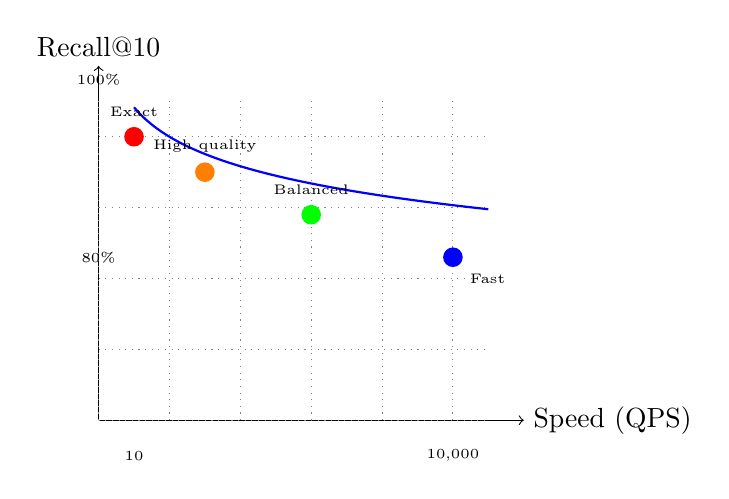
\begin{tikzpicture}[scale=0.9]
    % Axes
    \draw[->] (0,0) -- (6,0) node[right] {Speed (QPS)};
    \draw[->] (0,0) -- (0,5) node[above] {Recall@10};
    
    % Grid
    \draw[gray, dotted] (0,0) grid (5.5,4.5);
    
    % Curve
    \draw[blue, thick, domain=0.5:5.5, samples=100] 
        plot (\x, {4 - 0.6*ln(\x)});
    
    % Points
    \node[circle, fill=red, inner sep=2.5pt, label=above:{\tiny Exact}] at (0.5, 4) {};
    \node[circle, fill=orange, inner sep=2.5pt, label=above:{\tiny High quality}] at (1.5, 3.5) {};
    \node[circle, fill=green, inner sep=2.5pt, label=above:{\tiny Balanced}] at (3, 2.9) {};
    \node[circle, fill=blue, inner sep=2.5pt, label=below right:{\tiny Fast}] at (5, 2.3) {};
    
    % Labels
    \node at (0, 4.8) {\tiny 100\%};
    \node at (0, 2.3) {\tiny 80\%};
    \node at (0.5, -0.5) {\tiny 10};
    \node at (5, -0.5) {\tiny 10,000};
\end{tikzpicture}
